\section{Unsupervised Learning}
Das Ziel ist nicht eine Vorhersage, sondern Muster in den Daten zu erkennen und so die interne Struktur zu lernen.

\subsection{PCA}
Pricipal Component Analysis reduziert die Dimensionen. So müssen nicht $\frac{p(p-1)}{2}$ Scatter Plots gezeichnecht werden, für $p$ Dimensionen (oder Features). Dabei werden nur 1:1 Beziehungen geplottet.

Um die Prinzipal Components (PC) zu finden, müssen die Daten normalisiert sein ($x_i - \overline{x}= x_i$). Oft auch mit dem zScore $\frac{x_i - \overline{x}}{\sigma_x}= x_i$, um die Einheiten zu entfernen (andernfalls werden Äpfel mit Orangen verglichen). Der erste PC ist der Vektor, mit der grössten Varianz.
\begin{center}
	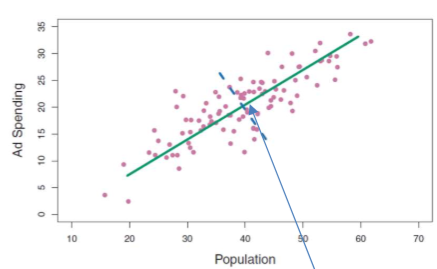
\includegraphics[width=0.7\columnwidth]{Images/pc}
\end{center}
Der zweite PC muss unkorreliert (orthogonal) zur ersten PC sein und ist wieder eine Linearkombination von $X_p$ mit maximaler Varianz.
\begin{center}
	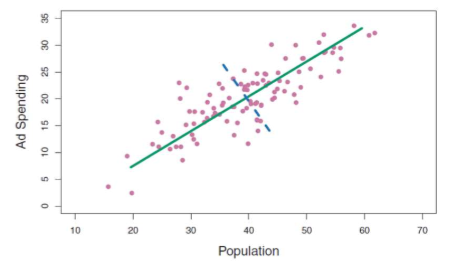
\includegraphics[width=0.7\columnwidth]{Images/pc2}
\end{center}

Um nun zu erfahren, wieviel Informtion jede PC vom gesammten Datenset enthält, kann Proportion of Variance Plot verwendet werden.

\begin{center}
	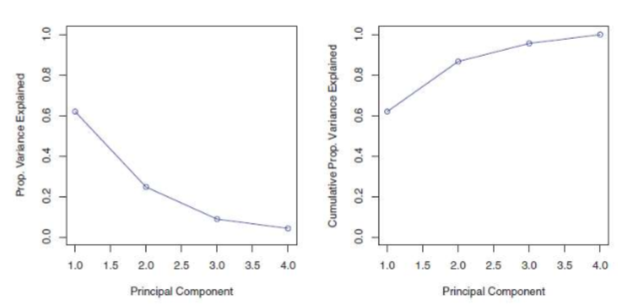
\includegraphics[width=\columnwidth]{Images/pc3}
\end{center}


\subsection{Clustering}\script{385}
Teilt das Datenset in $K$ Klassen mit $k$-means ein. Je besser die Klassen, desto kleiner die Varianz inherhalb des Clusters. 
\begin{center}
	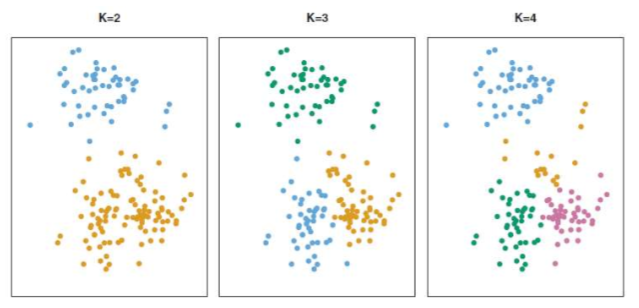
\includegraphics[width=0.5\columnwidth]{Images/clustering}
\end{center}

Dabei wird ein Dendogram generiert
\begin{center}
	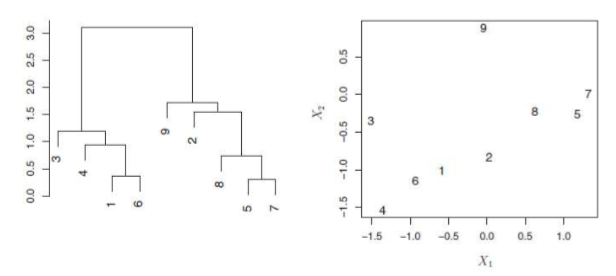
\includegraphics[width=\columnwidth]{Images/dendogram}
\end{center}

Es gibt unterschliedliche Typen, um ein Dendogram zu generieren. Leider beeinflusst der Type stark das Clustering, was das entscheiden des korrekten Types schwierig macht. Average und Complete tendieren zu balacierteren Dendrogrammen. Bei Single Linkages können jedoch jede Anzahl von Klassen gewählt werden. Der Vorteil von Centroid ist, dass dieser Schnell ist, und somit oft bei grössen $p$ verwendet wird, hat aber das Problem von Inversion.
\begin{center}
	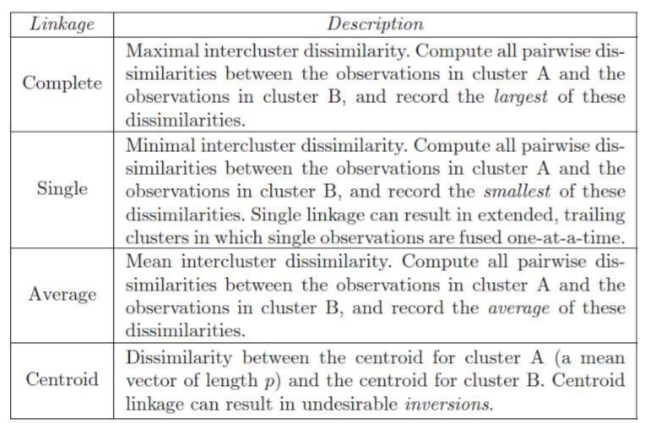
\includegraphics[width=\columnwidth]{Images/dendogram1}
\end{center}
